\subsection{Hard Debasing}
\subsection{Debiasing Conceptor}
\subsection{DensRay}
DensRay is an analytical method for identifying the
embedding subspace of certain linguistic features. Similar to the
methods mentioned in the previous section, we aim to
identify the ``gender subspace'' using a set of gendered words
$V:=\{v_1,v_2,\dots,v_n\}$ and their embeddings $E \in
R^{n\times d}$, thus for word $v_i$ we have the
corresponding embedding vector $e_{v_i}$. We
introduce a function $l$ for the gender attribute:
$l:V\to \{-1,1\}$;
e.g. $l(father)=1$, $l(sister)=-1$. The objective of DensRay
is to find an orthogonal matrix $Q\in R^{d\times d}$ such
that $EQ$ is gender-interpretable, specifically, the first
$k$ dimensions can be interpreted as the gender subspace.

Let $L_{=}:=\{(v,w)\in V\times V|l(v)=l(w)\}$ and define
$L_{\neq}$ analogously.  The DensRay objective
in \eqref{densray1} is to maximize the distance of the word
pairs from the same gender group ($L_{=}$) and minimize the
distance of the word pairs from the different gender group
($L_{\neq}$).
\begin{eqnarray}
\max\limits_{q} 
\sum_{(v,w)\in L_{\neq}}\alpha_{\neq}||q^Td_{vw}||^2_2
-\sum_{(v,w)\in L_{=}}\alpha_{=}||q^Td_{vw}||^2_2
\eqlabel{densray1}
\end{eqnarray}
where we define $d_{vw}:=e_v-e_w$. We also have $q\in R^d$
and $q^Tq=1$ since $Q$ is orthogonal. $\alpha_{\neq},\alpha_{=}\in [0,1]$ are hyperparameters. Observing that $||x||^2_2=x^Tx$, objective \eqref{densray1} can be simplified to:
\begin{eqnarray}
\max \limits_{q} q^T(
\sum_{(v,w)\in L_{\neq}}\alpha_{\neq}||d_{vw}d_{vw}^T||^2_2-\sum_{(v,w)\in L_{=}}\alpha_{=}||d_{vw}d_{vw}^T||^2_2)q=:\max\limits_{q} q^TAq
\label{eq:densray2}
\end{eqnarray}

The objective in \eqref{eq:densray2} is maximizing the Rayleigh quotient of $A$ and $q$. Since $A$ is symmetric, we can get an analytical solution $q$ by the eigenvector with the max eigenvalue of $A$ \shortcite{horn1990matrix}. Thus the matrix of $k$ eigenvectors of $A$ ordered by the corresponding eigenvalues yields the matrix $Q$.

\seclabel{artexample}
Here we compare the difference among DensRay, debiasing conceptor, and hard debiasing. \figref{fig:example} shows artificially created two dimensional embeddings. The lines show the gender directions identified by hard debiasing, conceptor and DensRay. Hard debiasing and conceptor does not use the labels of the male-female word pairs. Instead, hard debiasing relies upon the assumption that the first principal component of the considered vectors is a meaningful gender direction. This can fail in some cases. 

\enote{hs}{since this is a crucial point of the paper, we
	need a strong summary sentence here}


\begin{figure}[h]
	\centering
	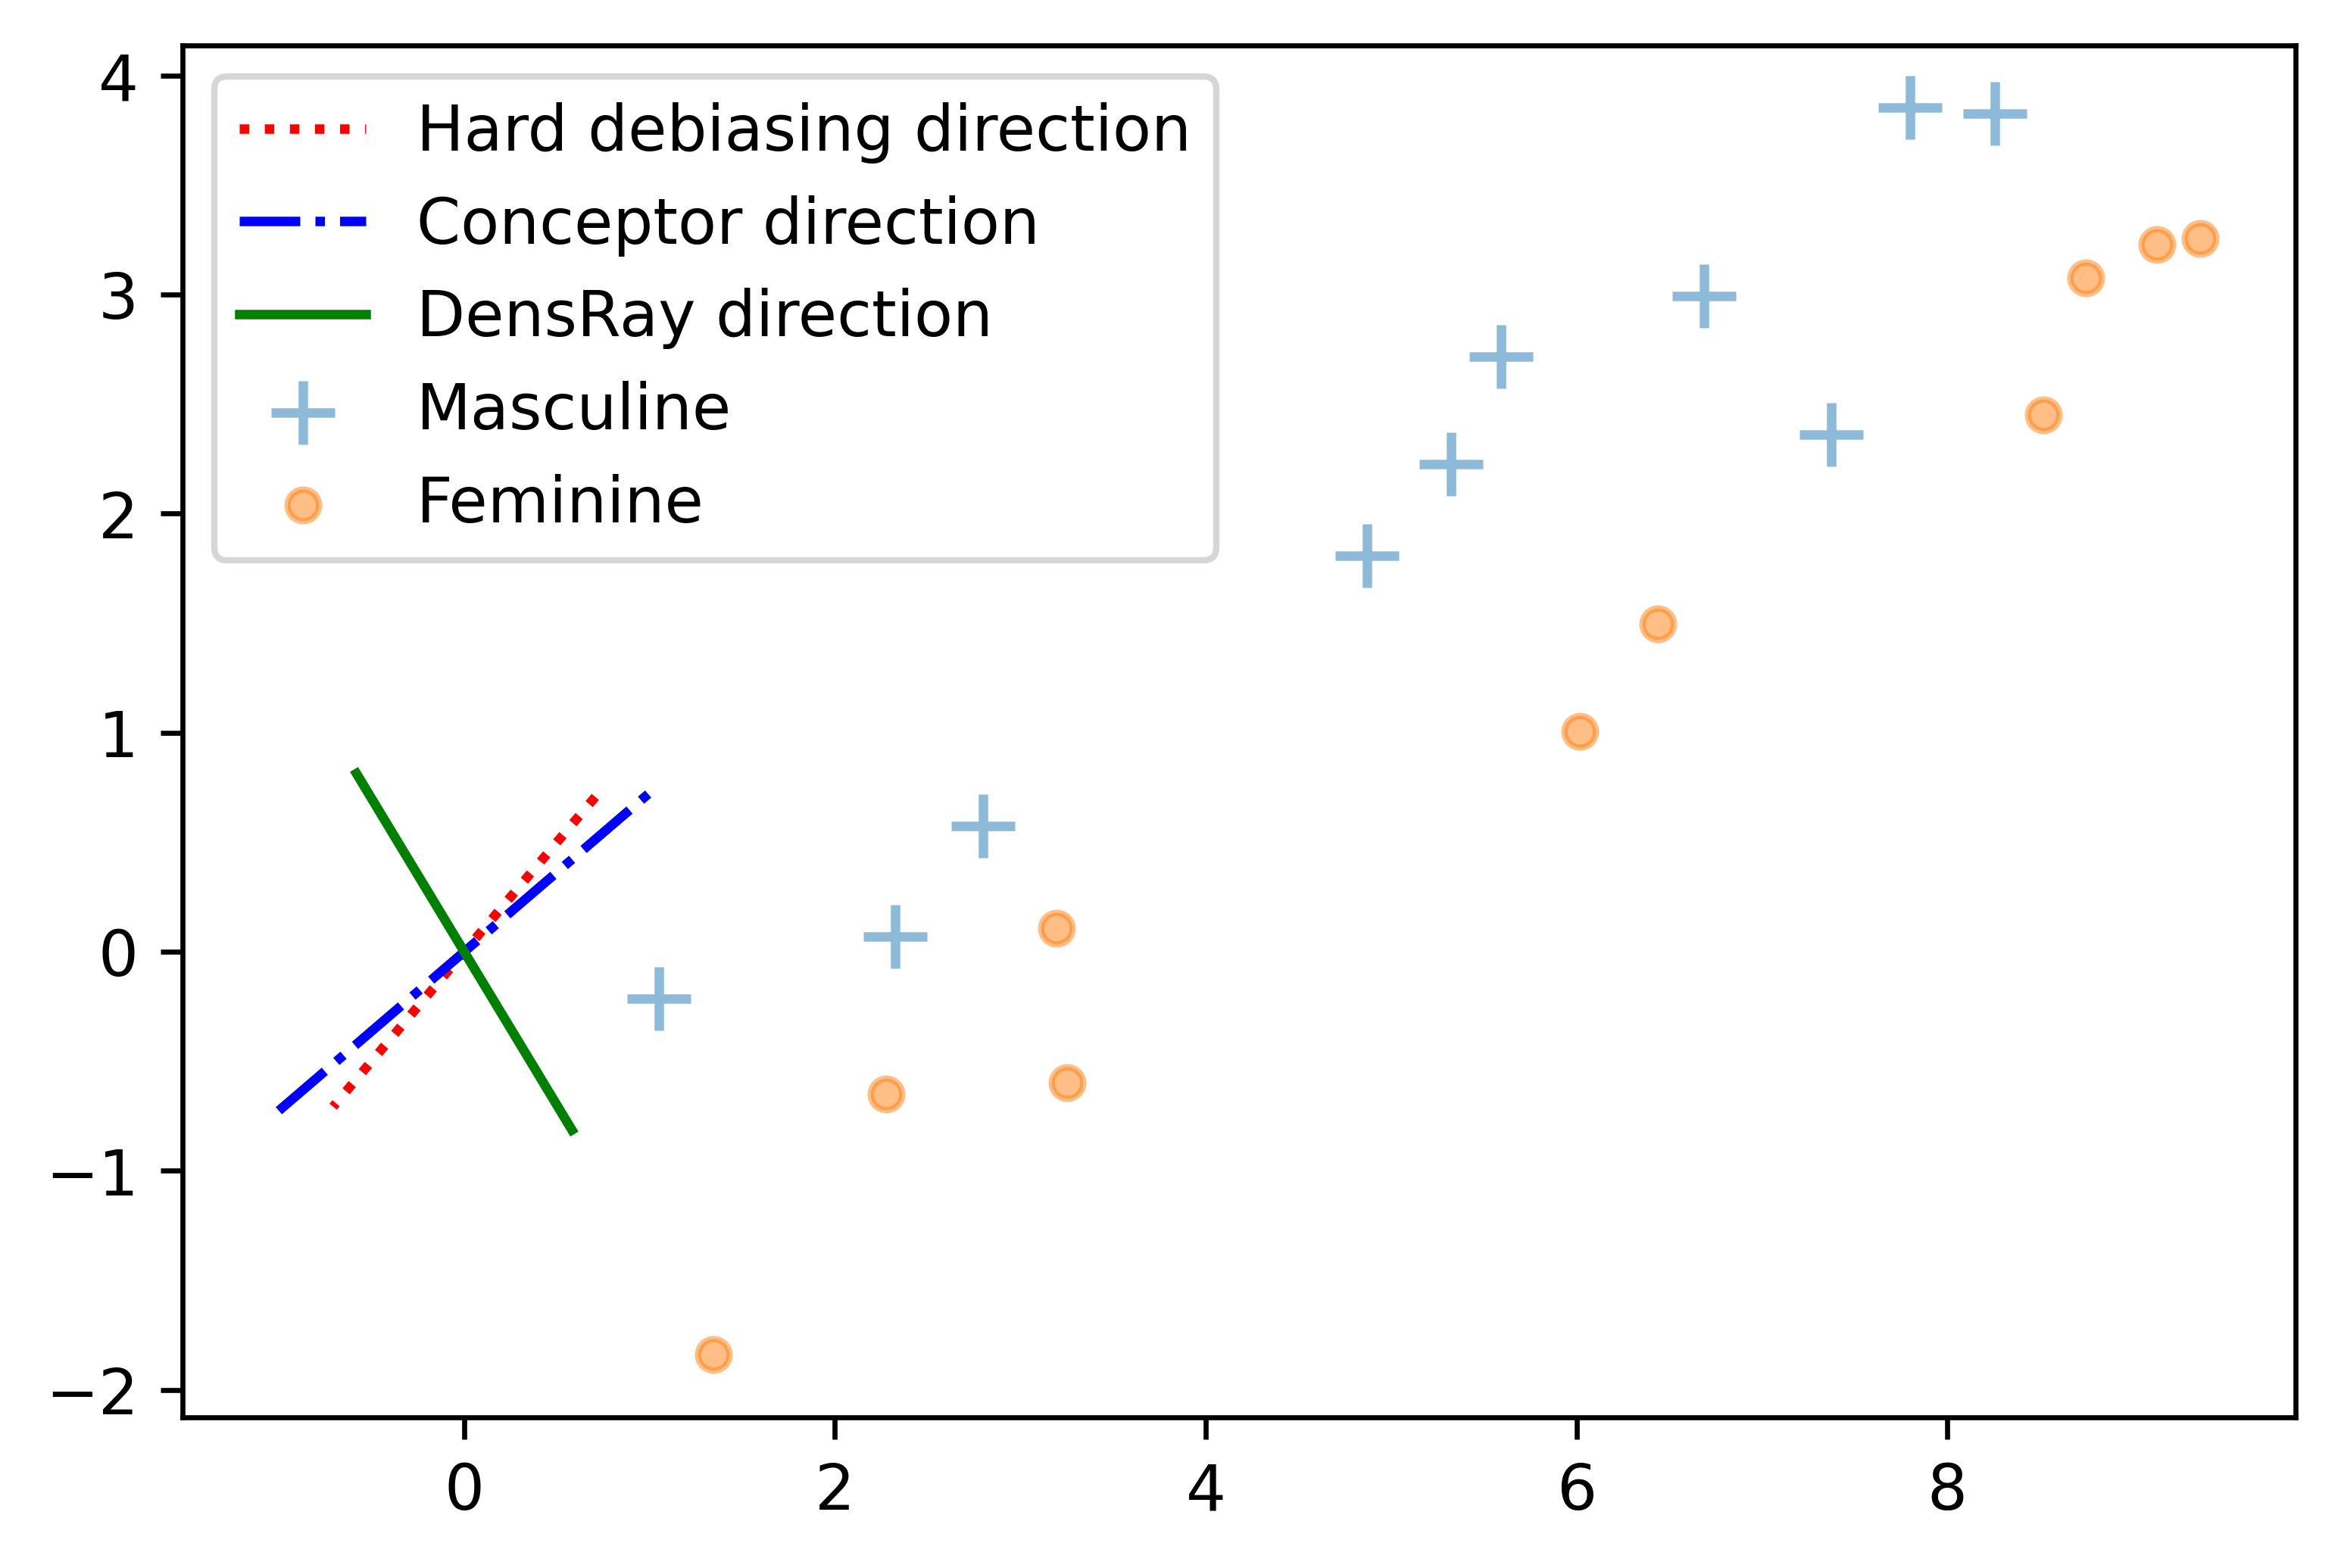
\includegraphics[width=0.9\linewidth]{examples.png}
	\caption{Gender direction on gendered words.}
	\figlabel{fig:example}
\end{figure}

\subsection{Adapting DensRay to Contextualized Language Models}
We now describe how we adapt DensRay to contextualized
language models. Given a set of gendered words
$V$, we extract sentences containing a word in $V$ from a
corpus. We run a contextualized language model
with $M$ layers
on each
sentence
$t_1,\ldots,t_j,\ldots,t_n$ (where $t_j \in V$)
and compute the contextualized representations $e^m, 1\leq m
\leq M$ of $t_j$, one for each layer. 
We compute an orthogonal rotation
matrix $Q_m$ for the $m$th BERT layer using Eq.\
\ref{eq:densray2}.
Finally, for debiasing, we set the dimensions
of the gender subspace to $0$ with the goal of eliminating or at least reducing gender
information that may cause bias; for measuring bias, we use the distance to the zero point of the gender subspace as the measurement. In this paper, we take the first dimension of the rotated space as the gender subspace.

